% ------- Flag di Debug  ---------------------------------------------------------------------------
\newif\ifToninus
\newcommand{\comment}[1]{\ifToninus\textcolor{gray}{\small{\textit{#1}}}\fi}
%\Toninustrue

%- D0cum3nt ----------------------------------------------------------------------------------------------------------------------------------
\ifToninus
\documentclass[8pt,handout]{beamer}
\else
\documentclass[9pt,handout]{beamer}
\fi

%- T1tle--------------------------------------------------------------------------------------------------------------------------
	\title{ Approccio Geometrico al metodo di Peierls e (Pre-)Quantizzazione del campo di Jacobi.}
	\author{Antonio Michele Miti}
	\date{20 novembre 2015}

%- Packages ---------------------------------------------------------------------------------------------------------------------------
%			Standalone non funziona ancora bene con beamer.
\usepackage[mode=buildnew]{standalone}				%\includestandalone[width=\textwidth]{Pictures/GeometricPicture0}
\usepackage{tikz}
\usepackage{pgfplots}
\pgfplotsset{compat=newest}
\usepackage{amsfonts}
\usepackage{xcolor}
\usepackage[utf8]{inputenc}
%\usepackage{fourier}							%\bomb \danger symbol
%\usepackage{arev}								%\smileface \sadface
\usepackage{animate}

%--Beamer Style--------------------------------------------------------------------------------------------------------------------------------
\usetheme{Copenhagen}

% FootLine
\setbeamertemplate{footline}[frame number]

%Headline
\setbeamertemplate{headline}{%
\leavevmode%
  \hbox{%
    \begin{beamercolorbox}[wd=\paperwidth,ht=2.5ex,dp=1.125ex]{palette quaternary}%
    \insertsectionnavigationhorizontal{\paperwidth}{}{\hskip0pt plus1filll}
    \end{beamercolorbox}%
  }
}

%Navigation Bar
\beamertemplatenavigationsymbolsempty



%Common symbols
%Common math symbols
	%Number fields
		\newcommand{\Real}{\mathbb{R}}
		\newcommand{\Natural}{\mathbb{N}}
		\newcommand{\Relative}{\mathbb{Z}}
		\newcommand{\Rational}{\mathbb{Q}}
		\newcommand{\Complex}{\mathbb{C}}
	
%equality lingo
	%must be equal
		\newcommand{\mbeq}{\overset{!}{=}} 

% function
	%Domain
		\newcommand{\dom}{\mathrm{dom}}
	%Range
		\newcommand{\ran}{\mathrm{ran}}
	

% Set Theory
	% Power set (insieme delle parti
		\newcommand{\PowerSet}{\mathcal{P}}

%Differential Geometry
	% Atlas
		\newcommand{\Atlas}{\mathcal{A}}
	%support
		\newcommand{\supp}{\textrm{supp}}

	
	
%Category Theory
	%Mor set http://ncatlab.org/nlab/show/morphism
%		\newcommand{\hom}{\textrm{hom}}

%Geometric Lagrangian Mechanics
	% Kinematic Configurations
		\newcommand{\Conf}{\mathtt{C}}
	%Solutions Space
		\newcommand{\Sol}{\mathtt{Sol}}
	%Lagrangian class
		\newcommand{\Lag}{\mathsf{Lag}}
	%Lagrangiana
		\newcommand{\Lagrangian}{\mathcal{L}}
	%Data
		\newcommand{\Data}{\mathsf{Data}}
	%unique solution map
		\newcommand{\SolMap}{\mathbf{s}}
	%Classical Observables
		\newcommand{\Obs}{\mathcal{E}}	
	%Phase Space
		\newcommand{\Phase}{\mathcal{M}}	

		\
		
%Peierls (per non sbagliare più)
		\newcommand{\Pei}{Peierls}
%---------------------------------------------------------------------------------------------------------------------------------------------------------------------

%\usetheme{CambridgeUs}





\begin{document}


%\/\/\/\/\/\/\/\/\/\/\/\/\/\/\/\/\/\/\/\/\/\/\/\/\/\/\/\/\/\/\/\/\/\/\/\/\/\/\/\/\/\/\/\/\/\/\/\/\/\/\/\/\/\/\/\/\/\/\/\/\/\/\/\/\/\/\/\/\/
%				Intro
%\/\/\/\/\/\/\/\/\/\/\/\/\/\/\/\/\/\/\/\/\/\/\/\/\/\/\/\/\/\/\/\/\/\/\/\/\/\/\/\/\/\/\/\/\/\/\/\/\/\/\/\/\/\/\/\/\/\/\/\/\/\/\/\/\/\/\/\/\/
%\section*{Intro}	

\ifToninus
%	\frame{\titlepage}
\else
	\frame{\titlepage}
\fi

\ifToninus
%	
\else
%	\begin{frame}{Overview}
%		(struttura della tesi vs struttura della presentazione)
%		\tableofcontents
%	\end{frame}
\fi


	

%\/\/\/\/\/\/\/\/\/\/\/\/\/\/\/\/\/\/\/\/\/\/\/\/\/\/\/\/\/\/\/\/\/\/\/\/\/\/\/\/\/\/\/\/\/\/\/\/\/\/\/\/\/\/\/\/\/\/\/\/\/\/\/\/\/\/\/\/\/
%				Parte 1 : 	"Foundations of Mechanics"
%\/\/\/\/\/\/\/\/\/\/\/\/\/\/\/\/\/\/\/\/\/\/\/\/\/\/\/\/\/\/\/\/\/\/\/\/\/\/\/\/\/\/\/\/\/\/\/\/\/\/\/\/\/\/\/\/\/\/\/\/\/\/\/\/\/\/\/\/\/		
	\section{Meccanica Geometrica}
\ifToninus
%
\else
%		\frame{\sectionpage}
\fi
		
	\begin{frame}	% \danger : manca immagine
		\frametitle{Formalismo canonico Ordinario (Finiti Gradi di Libertà)}
  			\begin{columns}[T]
    			\begin{column}{.5\textwidth}
						\begin{enumerate}
							\item\emph{Coordinate di Configurazione} $q^j$.
							\item\emph{Momenti Canonici Coniugati}  $p^j$.
							\item \emph{Matrice Simplettica} \comment{(combinando $p^i,q^j$ in un'unica variabile $Q^I=\{q_1,\ldots, q_N ;p^1, \ldots, p^N\}$)}
								\begin{displaymath}
									\Omega=\begin{bmatrix}
										\begin{matrix}0 & 1\\ -1 & 0\end{matrix} & & 0 \\
											 & \ddots & \\
											 0 & & \begin{matrix}0 & 1 \\ -1 & 0
										\end{matrix}
									\end{bmatrix}
								\end{displaymath}
							\item \emph{Parentesi di Poisson}: \comment{per 2 funzioni $A(Q^I) , B(Q^J)$}
								\begin{displaymath}
									\left\{A , B \right\} = \Omega^{I J} \frac{\partial A}{\partial Q^I} \frac{\partial B}{\partial Q^J}					
								\end{displaymath}
							\item \emph{Dinamica}
								\begin{displaymath}
									\left\{Q^I, H \right\} = \dot{Q}^I
								\end{displaymath}
							
								\comment{$$H(q,p) =  q \dot{q}(q,p)-L\left(q, \dot{q}(q,p)\right)$$}
								
								
						\end{enumerate}
    			\end{column}
    		   	\begin{column}{.5\textwidth}
					\parbox[c][.7\textheight][c]{\columnwidth}{%
						\comment{Animazione Pendolo con orbita rappresentata nel piano simplettico}
						\animategraphics[autoplay,loop,width=\textwidth]{3}{./Presentazione/SimpleHarmonicMotion/o_2830a51e4d07c739-}{0}{19}
 						\center \footnote{Fonte: 
 							\href{https://en.wikibooks.org/wiki/A-level_Physics_(Advancing_Physics)/Simple_Harmonic_Motion}{en.wikibooks.org}}
  					}	
    			\end{column}
  			\end{columns}	
		\end{frame}

	\begin{frame}	% \danger : manca overlay: popup graduale degli elementi
		\frametitle{Formalismo canonico Intrinseco}
  			\begin{columns}[T]
    			\begin{column}{.5\textwidth}
    				\comment{Il formalismo a cui siamo abituati può essere visto in modo intrinsecamente generale globale usando gli strumenti  della geometria differenziale, varietà e spazi tangenti}
						\begin{enumerate}
							\item Spazio di configurazione $Q$. \comment{(le coordinate di configurazione sono un sistema di coordinate (non dire "carte locali".)}
							\item Spazio delle velocità generalizzate $TQ$. \comment{incollando tutti gli spazi tangenti}
							\item Spazio delle fasi $T^*Q$. \comment{l'analogo per gli spazi duali, $Q^I$ sono una trivializzazione locale naturale)}
							\item $T^*Q$ è naturalmente simplettico $\omega = dp^i \wedge dq^i$.
							\item Dinamica codificata nelle funzioni $L$, $H$.\comment{Su TM è ambientata la dinamica lagrangiana e su T*M hamiltoniana.\\ sotto opportune condizioni sono equivalenti, }
						\end{enumerate}
    			\end{column}
    		   	\begin{column}{.5\textwidth}
    		   		\parbox[c][.7\textheight][c]{\columnwidth}{%
						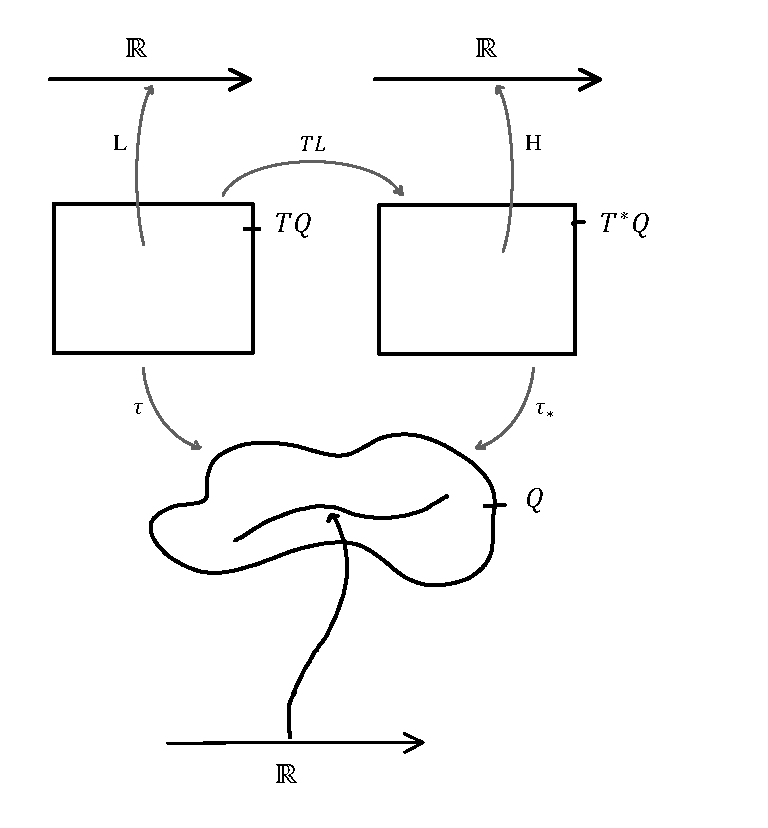
\includegraphics[width=\textwidth]{Presentazione/GeoMecFrameA} 
					}
    			\end{column}
  			\end{columns}	
		\end{frame}
		
		\begin{frame}	
			\frametitle{Formalismo Canonico Covariante}
  			\begin{columns}[T]
    			\begin{column}{.5\textwidth}
    				\comment{ Facciamo un Cambio di prospettiva: non più conformazioni "statiche" ma considero tutti i moti possibili}
					\begin{itemize}
						\item Spazio delle configurazioni cinematiche $\Conf$. \comment{è l'insieme di tutte i moti compatibili con la cinematica}
						\item Dinamica codificata dall'azione $S:\Conf \rightarrow \Real$. \comment{l'azione la rivediamo come una mappa definita sui moti}
						\item Equazioni differenziali del moto $ P$. \comment{ dal principio di minima azione discende un'equazione differenziale su $\Conf$}
						\item Spazio delle configurazioni dinamiche $\Sol$. \comment{Insieme delle equazioni del moto}		
					\end{itemize}

    			\end{column}

    		   	\begin{column}{.5\textwidth}
					\parbox[c][.7\textheight][c]{\columnwidth}{%
						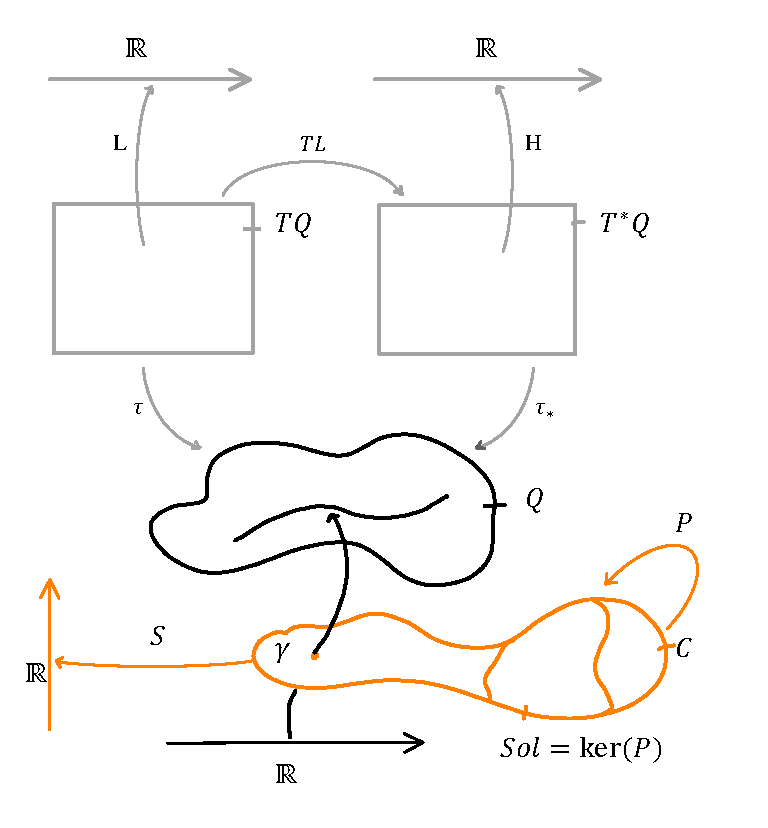
\includegraphics [width=\textwidth]{Presentazione/GeoMecFrameB} 
					}
    			\end{column}
  			\end{columns}		
		\end{frame}
	
		\begin{frame}	% \danger : manca overlay: popup graduale degli elementi
			\frametitle{Formalismo Covariante esteso ai Campi}
  			\begin{columns}[T]
    			\begin{column}{.5\textwidth}
    				\comment{Il formalismo covariante intrinseco si estende facilmente a sistemi più generali!\\}
    				L'idea:
    					\begin{itemize}
    						\item Insieme delle configurazioni:
    						    \begin{displaymath}
    								\underset{(\textrm{Spazio})}{Q} \quad \mapsto \quad 
    								\underset{(\textrm{Fibrato})}{\Real \times Q}
    							\end{displaymath}
    						\comment{La cinematica non viene più fondata su  $Q$ ma su $\Real \times Q$ (fibrato di configurazione) 	triviale nel caso dei sistemi ordinari}
    						\item Le configurazioni cinematiche: 
    							\begin{displaymath}
    								\underset{(\textrm{curve})}{\gamma: \Real \rightarrow Q} \quad \mapsto \quad 
    								\underset{(\textrm{sezioni})}{\gamma: \Real \rightarrow \Real\times Q}
    							\end{displaymath}
    					\end{itemize}	

    				\begin{block}<2->{Per  i campi}
 						\begin{itemize}
 							\item La varietà base è generico spaziotempo $M$.
 							\comment{La varietà base non è più $\Real$ ma un generico spaziotempo}
							\item Le configurazioni cinematiche sono mappe $\gamma: M \rightarrow M \times F$.
								\comment{$F$ è lo spazio target dei possibili valori che può assumere il campo}
							\item Equazioni del moto $P$ si rivacano da una \emph{Densità Lagrangiana} $\Lagrangian$ \comment{ingloba la struttura dinamica}
							\item Le configurazioni dinamiche sono le soluzioni di $P$
						\end{itemize}   				
    				\end{block}
    			\end{column}
    		 
    		   	\begin{column}{.5\textwidth}
					\comment{Evidenziare uno alla volta gli oggetti che introduco}
						\includegraphics<1-> [width=\textwidth]{Pictures/FieMecFrame} \\
						\includegraphics<2-> [width=\textwidth]{Presentazione/AbstractFieldTheory(pezzotta)} 
    			\end{column}
  			\end{columns}		
		\end{frame}
		
		
%\/\/\/\/\/\/\/\/\/\/\/\/\/\/\/\/\/\/\/\/\/\/\/\/\/\/\/\/\/\/\/\/\/\/\/\/\/\/\/\/\/\/\/\/\/\/\/\/\/\/\/\/\/\/\/\/\/\/\/\/\/\/\/\/\/\/\/\/\/
%				Parte 2 : 	"L'algoritmo di Peierls"
%\/\/\/\/\/\/\/\/\/\/\/\/\/\/\/\/\/\/\/\/\/\/\/\/\/\/\/\/\/\/\/\/\/\/\/\/\/\/\/\/\/\/\/\/\/\/\/\/\/\/\/\/\/\/\/\/\/\/\/\/\/\/\/\/\/\/\/\/\/		
%	\part{	Costruzione della struttura simplettica nel caso dei campi classici}
	\section{Metodo di Peierls}
\ifToninus
%
\else
%		\frame{\sectionpage}
\fi
	
	\begin{frame}{Il metodo di Peierls}
	    \begin{block}{Di cosa si tratta}
			\begin{itemize}
				\item Ricetta per definire forma bilineare sulle Lagrangiane.
					\comment{è una ricetta che permette di definire una forma bilineare sullo spazio delle Lagrangiane di un sistema lineare.}
				\item Ristretta ad un insieme opportuno risulta una buona forma simplettica.
					\comment{Fa discendere su un opportuno spazio di osservabili classici una struttura di poisson detta "parentesi di Peierls"}
			\end{itemize}
		\end{block}
	    \begin{block}{Prerequisiti \comment{Applicabilità del metodo di Peierls}}
			\begin{itemize}
				\item Teorie di Campo lineari
					\comment{:	$E=(E,\pi,M;Q)$ è un fibrato vettoriale, le equazioni del moto sono lineari.}
				\item Equazioni del moto ammettono funzioni di Green
					\comment{La dinamica è Lagrangiana con operatore del moto \emph{Green iperbolico} $P=Q_\Lagrangian$}
				\item Problema ai dati iniziali ben posto.
					\comment{ Lo spaziotempo sottostante permette di descrivere le soluzioni come un usuale problema sui dati iniziali (Lo spaziotempo sottostante è \emph{Globalmente iperbolico})}
			\end{itemize}
		\end{block}		
	\end{frame}
	
	\begin{frame}
		\frametitle{ Concetto chiave dell'algoritmo di Peierls : \underline{Disturbo Lagrangiano}}
			\comment{Le densità lagrangiane compatibili sono tante!\\Costituiscono uno spazio vettoriale di distribuzioni $\Lag$\\}
			Le densità Lagrangiane compatibili con la cinematica formano un insieme $\Lag$.\\
			Ognuna di esse possiede due statuti
			\comment{Ognuna di esse possiede essenzialmente due statuti}
			\begin{itemize}
				\item Può essere \emph{Motore della dinamica} \comment{(Determina l'operatore delle equazioni del moto)}
					\begin{displaymath}
						Q_\chi (\gamma) = \Biggr( \nabla_\mu \biggr( \frac{\partial \chi}{\partial(\partial_\mu \phi)} \biggr\vert_\gamma \biggr) - \frac{\partial \chi}{\partial \phi}\biggr\vert_\gamma \Biggr) \qquad \forall \gamma \in \Conf
					\end{displaymath}
				\item E' una quantità che può essere \emph{valutata} su una qualsiasi configurazione del sistema \comment{(Determina un funzionale Lagrangiano)}
					\begin{displaymath}
						\mathcal{O}_\Lagrangian [\phi] (f) = \int_M \Lagrangian [\phi] f \textrm{d}\mu
					\end{displaymath}	
			\end{itemize}
		\vfill
		\begin{exampleblock}{Ci chiediamo:}
			Come si modificano le configurazioni dinamiche del sistema quando la Lagrangiana viene disturbata da una seconda densità  $\chi$
			\begin{displaymath}
				\Lagrangian \rightsquigarrow \Lagrangian' = \Lagrangian + \epsilon\cdot \chi
			\end{displaymath}
		\end{exampleblock}
		\comment{Possiamo chiederci: \\
			Se la lagrangiana di un sistema fissato $(E,\Lag)$ viene alterata per un intervallo di tempo definito \comment{(supporto "time-compact")} da una seconda quantità che chiamiamo \emph{"Disturbo Lagrangiano"}
			\begin{displaymath}
				\Lagrangian \rightsquigarrow \Lagrangian' = \Lagrangian + \epsilon\cdot \chi
			\end{displaymath}
			come cambiano le configurazioni dinamiche del sistema?}
		\end{frame}
	
		\begin{frame}{L'effetto del Disturbo Lagrangiano}
		  	\begin{columns}[T]
    			\begin{column}{.5\textwidth}
						\begin{itemize}
							\item Fissata una soluzione $\phi_0$ del sistema imperturbato \comment{ $(E, \Lagrangian)$}
							\item Un disturbo Lagrangiano $\chi$ determina univocamente due soluzioni \emph{"disturbate"}
								\begin{displaymath}
									\phi^\pm_\epsilon = \phi_0 + \epsilon \eta_\pm
								\end{displaymath}
								dove:
								 \begin{displaymath}
   									\eta_\pm = G^\pm \big( - Q_\chi \phi_0 \big)
   								\end{displaymath}
   								\comment{Dove $G^\pm$ sono gli unici operatori di green avanzati/ritardati associati all'operatore $P$ delle equazioni del moto imperturbate}
   						\item L'\emph{effetto} di un disturbo Lagrangiano su un funzionale $B:\Conf\rightarrow \Real$ è:
   							\begin{displaymath}		
								\EffectOp_\chi^\pm B ( \phi_0) 
								= \lim_{\epsilon \rightarrow 0}
								 \biggr( \frac{B(\phi_\epsilon^\pm) - B (\phi_0)}{\epsilon} \biggr)
   							\end{displaymath}			
						\end{itemize}
    			\end{column}
    		   	\begin{column}{.5\textwidth}
					\parbox[c][.7\textheight][c]{\columnwidth}{%
						% Your image included here
							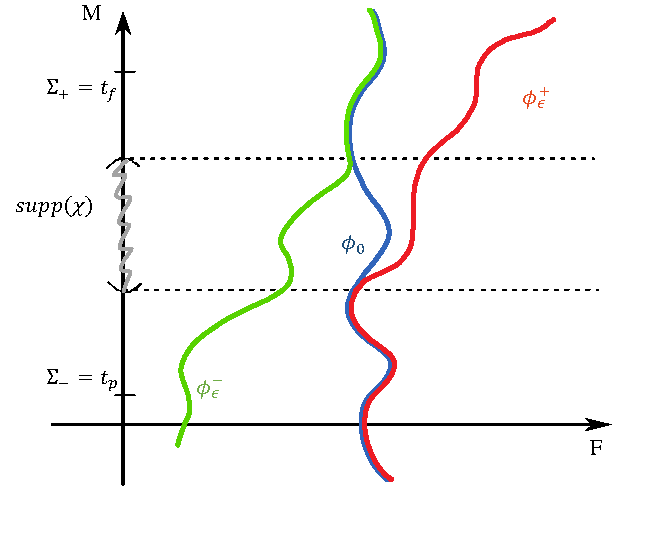
\includegraphics[width=\textwidth]{Presentazione/AdvRetSol(pezzotta)}
					}
    			\end{column}
    		\end{columns}
	\end{frame}

	\begin{frame}
		\frametitle{I passi del metodo di Peierls}
			Per semplicità rappresentiamo lo spazio infinito dimensionale $\Conf$ come un piano.
		  	\begin{columns}[T]
    			\begin{column}{.5\textwidth}
						\begin{enumerate}
							\item<2->  Alla  Lagrangiana disturbata corrisponde un proprio spazio di soluzioni.
							\item<3-> Si determinano tra tutte le possibili variazioni $\phi_\epsilon$ di $\phi_0$ quelle che ricadono in $\Sol_\epsilon$ al primo ordine in $\epsilon$
							\item<4-> L'effetto è la derivata del valore di un funzionale $B$ lungo le variazioni appena trovate.
							\item<5-> La parentesi di Peierls si ottiene per confronto dei due effetti anticipato e ritardato:
								\begin{displaymath}
									\{\chi, \omega \}(\phi_0) =
									 \EffectOp_\chi^- \mathcal{O}_\omega (\phi_0) - \EffectOp_\chi^+ \mathcal{O}_\omega(\phi_0)
								\end{displaymath}
						\end{enumerate}
    			\end{column}
    		   	\begin{column}{.5\textwidth}
								\includegraphics<1>[width=\textwidth]{Pictures/GeometricPicture0}
								\includegraphics<2>[width=\textwidth]{Pictures/GeometricPicture1}
								\includegraphics<3>[width=\textwidth]{Pictures/GeometricPicture2}								
								\includegraphics<4-5>[width=\textwidth]{Pictures/GeometricPicture3}
    			\end{column}
    		\end{columns}
	\end{frame}

	
	
%\/\/\/\/\/\/\/\/\/\/\/\/\/\/\/\/\/\/\/\/\/\/\/\/\/\/\/\/\/\/\/\/\/\/\/\/\/\/\/\/\/\/\/\/\/\/\/\/\/\/\/\/\/\/\/\/\/\/\/\/\/\/\/\/\/\/\/\/\/
%				Parte 3 : 	"Realizzazione Specifica del campo di Jacobi"
%\/\/\/\/\/\/\/\/\/\/\/\/\/\/\/\/\/\/\/\/\/\/\/\/\/\/\/\/\/\/\/\/\/\/\/\/\/\/\/\/\/\/\/\/\/\/\/\/\/\/\/\/\/\/\/\/\/\/\/\/\/\/\/\/\/\/\/\/\/		
	%\part{Realizzazione per il Caso specifico dei campi di Jacobi}
	\section{Campo di Jacobi}
\ifToninus
%
\else
%		\frame{\sectionpage}
\fi

	\begin{frame}
		\frametitle{ Ricordiamo il problema di Jacobi }
		  	\begin{columns}[T]
    			\begin{column}{.5\textwidth}
					\begin{itemize}
							\item<1-> Varietà \comment{una generalizzazione del piano cartesiano i.e. coordinatizzabile}
							\item<2-> Pseudo-Riemmanian \comment{Dotata di una metrica= forma bilineare simmetrica su ogni spazio tangente}
							\item<3-> \comment{in presenza di una metrica posso formulare il problema geodetico}
								Le geodetiche \comment{sono curve che} soddisfano l'equazione di lunghezza estremale \comment{ autoparallela rispetto la connessione di levi-civita\\}
								\begin{displaymath}
									\nabla_{\dot{\gamma}}\dot{\gamma} = \ddot{\gamma}^i + \Gamma^i_{\, j k} \dot{\gamma}^j \dot{\gamma}^k =0
								\end{displaymath}
							\item<4-> La variazione regolare di una curva $\gamma_0$ determina un campo lungo la curva.
							\item<5-> Una variazione geodetica determina un campo che soddisfa le equazioni di \emph{Jacobi}
								\comment{\\Catchword: campi di Jacobi come il moto di attrazione apparente di due gravi in caduta libera (fenomeno della deviazione geodetica)}
								\begin{displaymath}
									\big( X''\big)^\mu + R^\mu_{i \alpha \j} T^i X^\alpha T^j =0
								\end{displaymath}
					\end{itemize}
    			\end{column}
    		   	\begin{column}{.5\textwidth}
    		   		\parbox[c][.7\textheight][c]{\columnwidth}{%
						\includegraphics<1>[width=\textwidth]{Presentazione/LocalChart}
						 	\center \footnote<1>{Fonte: \href{http://kahrstrom.com/mathematics/illustrations.php}{http://kahrstrom.com/}}

						\only<1>{\comment{credit \url{http://kahrstrom.com/}}}
						\includegraphics<2>[width=\textwidth]{Presentazione/Sfera_Tangent}
						\only<2>{\comment{\\Wip: esibire la presenza di una distanza (come lunghezza della curva di minima lunghezza?)}}
						\includegraphics<3>[width=\textwidth]{Presentazione/Sfera_Main}
						\only<3>{\comment{\\Wip: esibire il problema geodetica come circonferenze massimali}}
						\only<4>{\animategraphics[autoplay,loop,width=\textwidth]{6}{./Presentazione/ParallelVariation}{}{}}
						\only<4>{\comment{\\Wip: esibireUn campo tangente lungo un meridiano}}
						\only<5>{\animategraphics[autoplay,loop,width=\textwidth]{6}{./Presentazione/GeodesicVariation}{}{}}
						\only<5>{\comment{\\Wip: animazione di una variazione Geodetica con campo Jacobi tangente alla variazione}}
					}
    			\end{column}
    		\end{columns}
	\end{frame}
	
	\begin{frame}
		\frametitle{I Campi di Jacobi visti come un sistema fisico}
			\begin{block}{Cinematica}
				\comment{Il fibrato di configurazione $E$ corrisponde al \emph{fibrato pull-back} $\gamma_0^*(TQ)$ del fibrato tangente lungo la geodetica$\gamma_0$.\\
					 $E$ è un fibrato sulla retta $\Real$				
					}
					\begin{itemize}
						\item La varietà di base è $\Real$ 
							\comment{\\ è uno spazio globalmente iperbolico "triviale". \\ $\CauchyClass(\Real) = \Real$.}
				\item Le varietà di target \comment{Le fibre} sono $E_p = T_{\gamma_0(p)}Q$
				\item $\Conf = \Gamma^\infty(E) = \mathfrak{X}(\gamma_0)$ è costituito da campi lungo la curva $\gamma_0$.
					\end{itemize}
			\end{block}
			\begin{block}{Dinamica}

				\begin{itemize}
					\item Equazioni del moto: $ \left( P X \right)^\mu = (X'')^\mu + R^\mu_{\, i \alpha j } T^i T^j X^\alpha$ 
						\comment{				Dove $X\in \Conf$ e $T^i = \dot{\gamma_0}^i$.}
						\comment{ 					L'operatore del moto è \emph{Normalmente Iperbolico}}
				\end{itemize}
			\comment{\emph{Normalmente Iperbolico} è una condizione più forte di Green-hyperbolico. in questo caso sia la costruzione di Peierls che quella di Wald sono ben definite}

			\end{block}
	

			\begin{block}{Metodo di Peierls}
				\begin{itemize}
					\item Spazio degli osservabili classici:  $	\Obs \simeq \frac{\Gamma_0}{P \Gamma_0}$
					\item Funzionali associati: $ F_{[f]}(X) = F_f (X)= \int_\Real <X, f>_t dt \qquad \forall X \in \Sol $
					\item Parentesi di Peirels: 
						$ \left\lbrace\chi , \omega \right\rbrace = \int \left\langle\chi, \left(\GreenAdv - \GreenRet \right)\omega \right\rangle dt  
							= (\chi, E \omega)$
						\comment{$$ \left\lbrace\chi , \omega \right\rbrace (\gamma_0) [f] = \int f(t) \left\langle\chi, \left(\GreenAdv - \GreenRet \right)\omega \right\rangle dt $$}
				\end{itemize}
			\end{block}
	\end{frame}
	



\begin{frame}{Lo spazio delle Fasi Classico}
					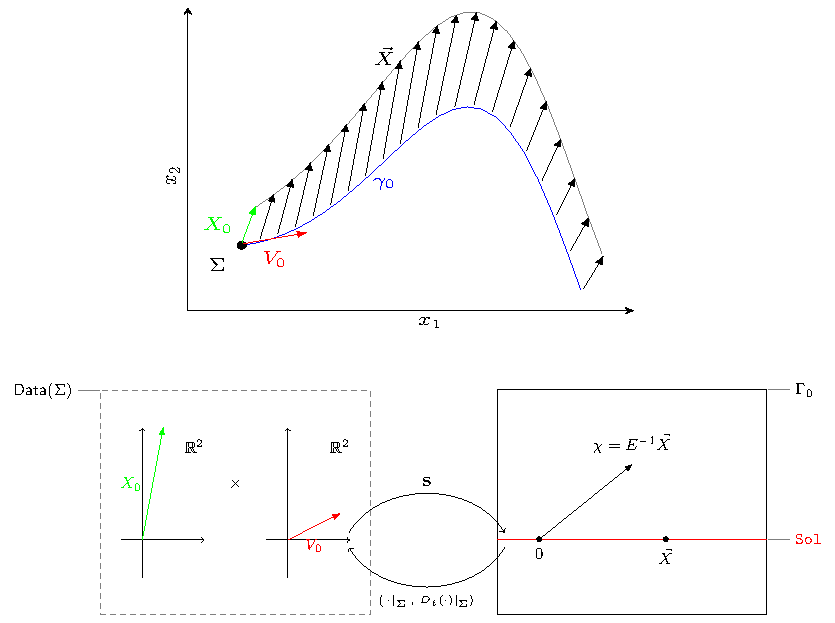
\includegraphics[width=\textwidth]{Pictures/Jacobi_GeometricPicturePanoramica}	

\end{frame}	

	


%\/\/\/\/\/\/\/\/\/\/\/\/\/\/\/\/\/\/\/\/\/\/\/\/\/\/\/\/\/\/\/\/\/\/\/\/\/\/\/\/\/\/\/\/\/\/\/\/\/\/\/\/\/\/\/\/\/\/\/\/\/\/\/\/\/\/\/\/\/
%				Fine	!!!
%\/\/\/\/\/\/\/\/\/\/\/\/\/\/\/\/\/\/\/\/\/\/\/\/\/\/\/\/\/\/\/\/\/\/\/\/\/\/\/\/\/\/\/\/\/\/\/\/\/\/\/\/\/\/\/\/\/\/\/\/\/\/\/\/\/\/\/\/\/		
\section*{Conclusioni e Prospettive}

		\begin{frame}
		\frametitle{ Conclusioni}
			\begin{block}{Risultati}
				\begin{itemize}
					\item Riformulazione in linguaggio geometrico dell'algoritmo di Peierls.
					\item Estensione dell'algoritmo di Peierls da campi scalari a teorie di campo Lagrangiane su spaziotempo curvo.
				\end{itemize}
			\end{block}
			\begin{block}{Prospettive}
				\begin{itemize}
					\item Cercare un interpretazione geometrica ai singoli passaggi che costituiscono il metodo di Peierls.
					\comment{Ci si può porre il problema di trovare un interpretazione geometrica ai singoli passaggi che costituiscono il metodo di \emph{Peierls}.\\
				 Perché la costruzione di Peierls fornisce proprio la giusta usuale forma simplettica ($\Omega$) sullo spazio delle fasi classico ?}
					\item Riformulazione rigorosa delle costruzioni formali sviluppando un \emph{calcolo differenziale sulle varietà infinito dimensionali}.\comment{ con gli strumenti dell'\emph{analisi globale}.}
					\item Estensione ulteriore della procedura di Peierls a teorie più elaborate\\
					(Libertà di Gauge, Equazioni di Vincolo, Strutture di Spin).
					\item 	Formulazione della struttura geometrica che soggiace allo spazio delle Lagrangiane
						\comment{E' possibile fornire un'interpretazione geometrica alle parentesi di Peierls formalizzando lo spazio delle Lagrangiane?}
					\end{itemize}				 
			\end{block}
	\end{frame}


%\/\/\/\/\/\/\/\/\/\/\/\/\/\/\/\/\/\/\/\/\/\/\/\/\/\/\/\/\/\/\/\/\/\/\/\/\/\/\/\/\/\/\/\/\/\/\/\/\/\/\/\/\/\/\/\/\/\/\/\/\/\/\/\/\/\/\/\/\/
%				Parte 4 : 	Extra Backup Eliminata
%\/\/\/\/\/\/\/\/\/\/\/\/\/\/\/\/\/\/\/\/\/\/\/\/\/\/\/\/\/\/\/\/\/\/\/\/\/\/\/\/\/\/\/\/\/\/\/\/\/\/\/\/\/\/\/\/\/\/\/\/\/\/\/\/\/\/\/\/\/		
	\section{Extra}
	\frame{\sectionpage}	

		\begin{frame}{Meccanica Geometrica}
  			\begin{columns}[T]
    			\begin{column}{.5\textwidth}		
					\begin{itemize}
						\item \textbf{L'Idea:} Fare uso della geometria per codificare tutte le proprietà meccaniche di un sistema indipendentemente dalle coordinate di configurazione.(Lessig)
						\item \textbf{La scommessa:} Saper ricostruire da questi oggetti matematici astratti tutte le osservabili di interesse fisico.
						\item \textbf{Il vantaggio:} Base formale su cui definire la Quantizzazione.
					\end{itemize}
    			\end{column}
    		   	\begin{column}{.5\textwidth}
							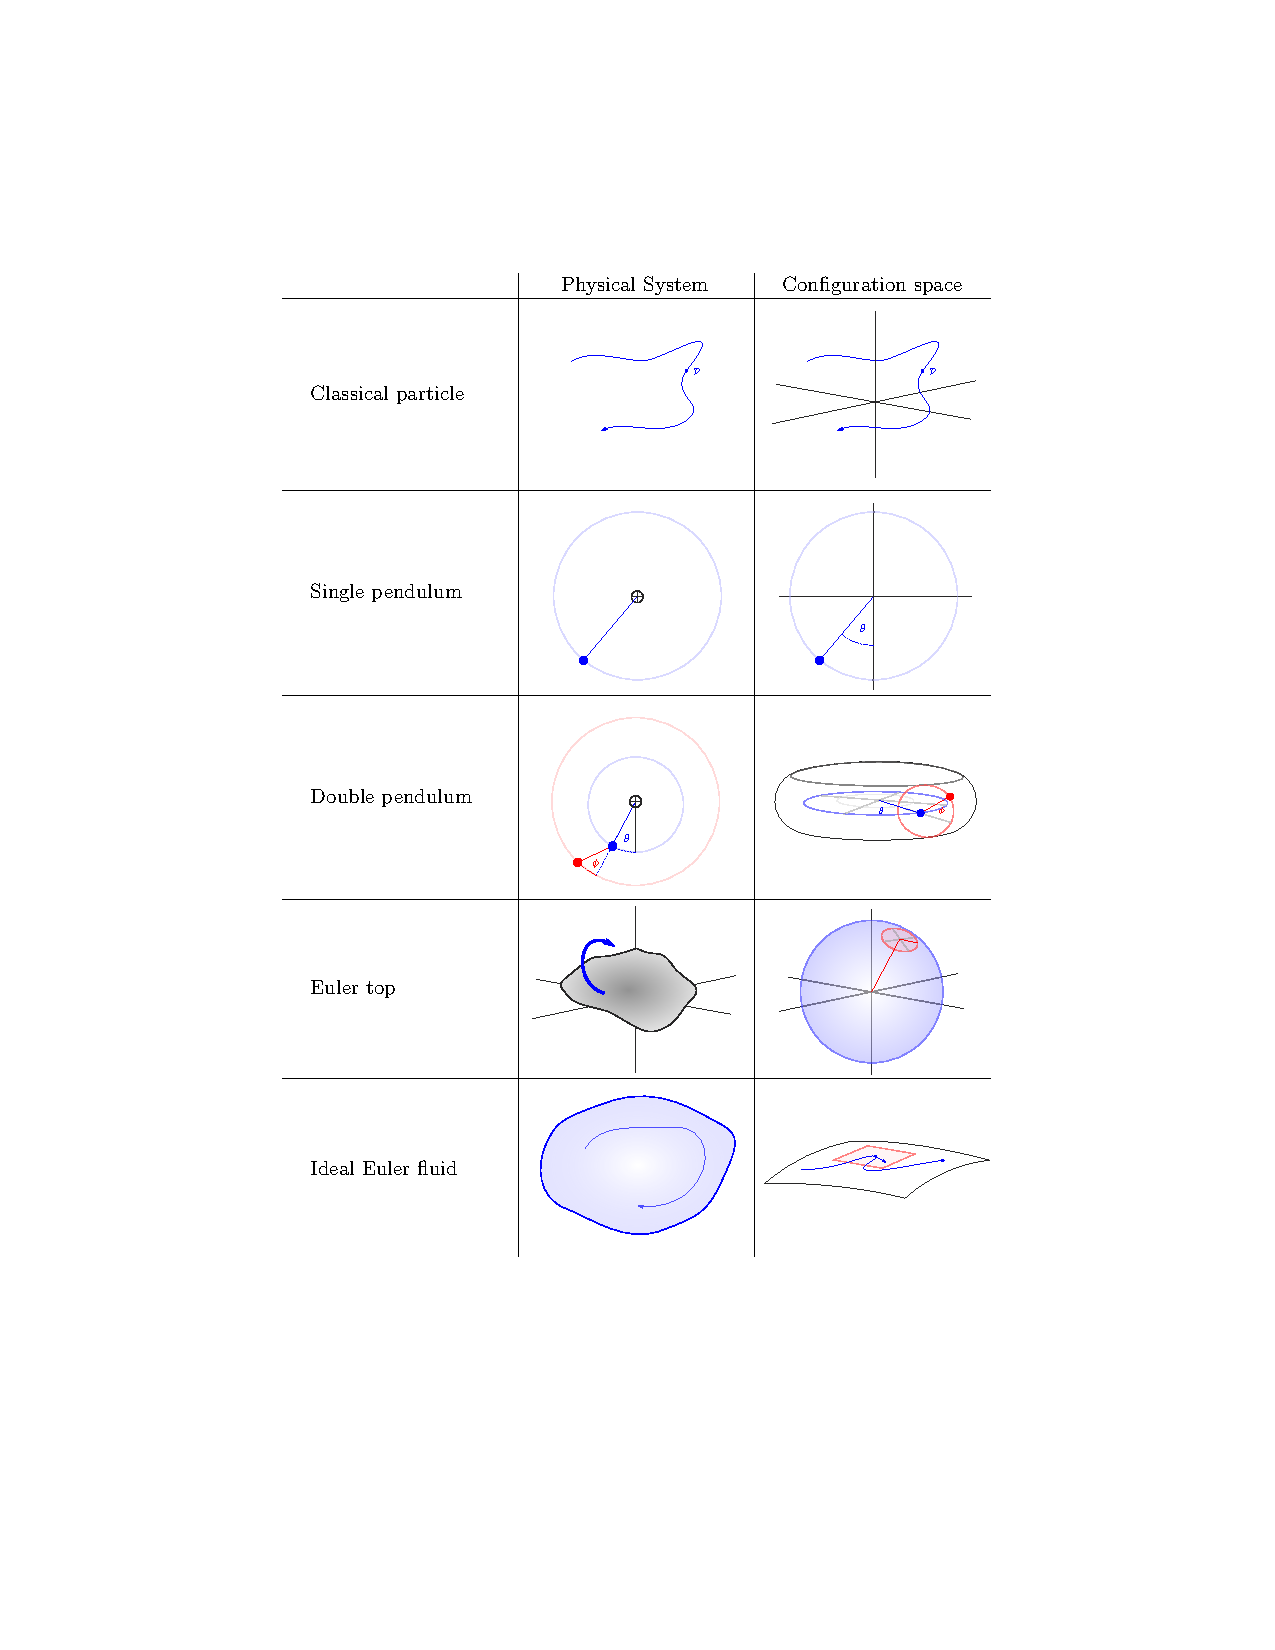
\includegraphics[width=\textwidth]{Presentazione/GeoMec_Crop} 		
							 \center \footnote{Fonte: 
 								\href{http://arxiv.org/abs/1206.3302}{\emph{A Primer on Geometric Mechanics} - C. Lessig}
  							}	
    			\end{column}
  			\end{columns}	
	\end{frame}

	\begin{frame}
		\frametitle{I passi del metodo di Peierls (1)}	
			La procedura può essere riassunta in pochi passi:
		\begin{enumerate}
			\item Si considera un disturbo Lagrangiano$\chi$. \comment{that is a time-compact Lagrangian density}
			\item Si costruiscono le soluzioni perturbate dall'azione di $\chi$.
			\item Si calcolo l'effetto del disturbo $\chi$ sul funzionale Lagrangiano relativo ad un secondo disurbo $\omega$.
			\item Si assembla l'effetto reciproco dei due disturbi a costruire una funzione binaria.
		\end{enumerate}	
	\end{frame}

	\begin{frame}{Dalle Parentesi di Peierls alla struttura simplettica \comment{sarebbe più corretto dire di Poisson}}
		\comment{Per semplicità mi riferisco ad un campo scalare}
		  	\begin{columns}[T]
    			\begin{column}{.5\textwidth}
						\begin{enumerate}
							\item Considero solo le Lagrangiane costruibili a partire da una configurazione cinematica. \comment{ osservabile sono le configurazioni a supporto compatto $\Gamma_0$.}
								\comment{la valutazione dell'osservabile $\chi \in \Gamma_0$ risulta:}
								\begin{align*}
									Q_\chi (\psi) &= -\chi \\
									\mathcal{O}_\chi (\psi) &= \int_M \chi(x) \psi(x) d\mu(x) = \left(\chi , \psi \right)
								\end{align*}
							\item<2-> Le soluzioni dell'equazione del moto disturbato
								\begin{displaymath}
									\Sol_\epsilon = \Sol + \epsilon \GreenAdv \chi =  \Sol + \epsilon \GreenRet \chi
								\end{displaymath}
							\item<3->	\comment{In questo caso i vettori delle variazioni su una soluzione $\phi_0 \in \Sol $ sono indipendenti dalla soluzione di partenza}
								Le variazioni $\eta_\pm$ sono indipendenti dalla soluzione di partenza
								\begin{displaymath}
									\eta_\pm = G^\pm (- Q_\chi \phi_0 ) = G^\pm \chi
								\end{displaymath}
							\item<4-> Le parentesi risultano
								\begin{displaymath}
									 \{ \omega , \chi \} = \left( \omega ,(\GreenAdv - \GreenRet) Q_\chi \phi_0\right)  = \left( \omega , E \chi \right)
								\end{displaymath}	
						\end{enumerate}
    			\end{column}
    		   	\begin{column}{.5\textwidth}
    		   		    \parbox[c][.7\textheight][c]{\columnwidth}{%
						\includegraphics<1-2>[width=\textwidth]{Pictures/compsupp_GeometricPicture1}
						\includegraphics<3>[width=\textwidth]{Pictures/compsupp_GeometricPicture2}
						\includegraphics<4->[width=\textwidth]{Pictures/compsupp_GeometricPictureLinear}
						}
    			\end{column}
    		\end{columns}
	\end{frame}

	\begin{frame}{L'Algebra di Poison realizzata tramite il metodo di Peierls}
		Risultato:\\
		Alla generica teoria lagrangiana di campo $(E, \Lagrangian)$\\
		Viene associato lo spazio simplettico  $(\Obs, \tau)$ 
		\begin{itemize}
			\item $\Obs \simeq \frac{\Gamma_0}{P \Gamma_0} $
			\item $\tau( [\chi], [\omega]) = \{\chi , \omega \} =\int_M \left\langle\chi, \left(\GreenAdv - \GreenRet \right)\omega \right\rangle 
			d\mu(x) = ( \chi, E \omega) \qquad \forall \chi,\omega \in \Gamma_0(E)$
		\end{itemize}
		\comment{SI prende il quoziente per garantire che la forma sia non degenere\\} 		

		\vfill

		Gli elementi di $\Obs$ agiscono come osservabili:
				\begin{displaymath}
				 F_{[f]}(X) = F_f (X)= \int_M <X, f>_x d\mu(x) \qquad \forall X \in \Sol
				\end{displaymath}
		La forma $\tau$ può essere rivista come una parentesi di Poisson
				\begin{displaymath}
				 \left\{ F_{[f]},  F_{[g]} \right\} (X) = F_{[???]}(X)
				\end{displaymath}
				\comment{adesso mi sfugge}
			
	\end{frame}


	\begin{frame}{Che c'entra tutto ciò con la quantizzazione?}
		Una volta determinato lo spazio simplettico classico della teoria di campo lo schema di quantizzazione si completa in due passi:
		\begin{enumerate}
			\item Si associa a $(\Obs, \tau)$ un'opportuna  "unital $\ast-$algebra". \comment{encoding the structural relations between the observables, such as causality and locality}
			\item Si seleziona uno stato algebrico \comment{ that is a positive, normalized, linear functional on the algebra which allows us to recover the standard probabilistic interpretation of quantum theories via the Gelfand-Neimark-Segal (GNS) theorem.} 
		\end{enumerate}
	\end{frame}
	
	\begin{frame}{L'algebra degli osservabili quantistici}
			We call \emph{algebra of quantum observables} associated to the classical field system $(\Obs, \tau)$ the unital $\ast-$algebra 
			$	\ObsAlg	= \big( (\ObsAlg, \Complex),\cdot,*\big)$ generated over $\Complex$ by the symbols 
			\begin{displaymath}
				\big\{\mathbf{1}\big\}\bigcup \big\{\mathbf{\Phi}\big( [f]\big) \; \big\vert \;  [f] \in \Obs \big\}
			\end{displaymath}
			such that:
			\begin{enumerate}
				\item The generators are linearly independent:
					\begin{equation}\label{Ip:GenIndip}
						\mathbf{\Phi} \big(a [f] + b [s] \big) = 
						a \mathbf{\Phi} ([f]) + b \mathbf{\Phi} ([s]) \qquad \forall [f],[s] \in \Obs,\: \forall a,b \in \Real
					\end{equation}
				\item The generators are \emph{formally self-adjoint} in the sense that:
					\begin{equation}\label{Ip:GenSelfAd}
						\big( \mathbf{\Phi}([f]) \big)^* = \mathbf{\Phi}([f]) \qquad \forall [f] \in \Obs
					\end{equation}
				\item The (anti-) commutation relations extrapolated from %....The rules of (anti-) commutation given from 
					the classical $\tau$ are replicated on $\ObsAlg$:
					\begin{equation}\label{Ip:ImplementCCR}
						\big[ \mathbf{\Phi}([f]), \mathbf{\Phi}([g]) \big]_\mp = \mathbf{\Phi}([f]) \cdot \mathbf{\Phi}([g]) \mp \mathbf{\Phi}([g]) \cdot \mathbf{\Phi}([f]) = i \tau\big( [f], [g] \big) \mathbf{1}
					\end{equation}
					where the sign $\mp$ depend respectively on the anti-symmetry and symmetry of the form $\tau$.
			\end{enumerate}
	\end{frame}
	
	\begin{frame}
		\frametitle{ Prospettive}
			\begin{itemize}
				\item Ci si può porre il problema di trovare un interpretazione geometrica ai singoli passaggi che costituiscono il metodo di \emph{Peierls}.\\
				 Perché la costruzione di Peierls fornisce proprio la giusta usuale forma simplettica ($\Omega$) sullo spazio delle fasi classico ?
				\item Tali costruzioni sono formali. E' possibile dare un fondamento rigoroso a tali costruzioni sviluppando il \emph{calcolo differenziale sulle varietà infinito dimensionali} \comment{Analisi Globale}
				\item E' possibile estendere ulteriormente la procedura di Peierls a teorie di campo più articolate?
					\begin{itemize}
						\item Libertà di Gauge
						\item Equazioni di Vincolo
						\item Strutture di Spin
					\end{itemize}
				\item Al discorso soggiace la geometria di 2 spazi: lo spazio delle soluzioni $\Sol$ e lo spazio delle Lagrangiane $\Lag$.\\
					E' possibile fornire un'interpretazione geometrica alle parentesi di Peierls formalizzando lo spazio delle Lagrangiane?
			\end{itemize}
	\end{frame}	
	
\end{document}

